\section{Model Architecture}
\label{sec:archi}

\subsection{Style Extractor}

스타일 이미지에서 스타일을 추출해내기 위해서, 우리는 ImageNet Classification Challenge \cite{Deng2009ImageNet}에서 우수한 성능을 보여준 학습된 VGGNet \cite{Simonyan2014}의 convolutional layer와 첫 번째 fully connected layer를 사용하였다.
이를 통해 Style Extractor를 통과한 224 x 224 크기의 이미지는 크기가 4096인 벡터가 되고, 우리는 이 벡터가 스타일 이미지의 스타일 정보를 가지고 있을 것이라는 판단을 하였다.
\subsection{Generator}

Generator 모델은, 가장 기본적으로는 \stylepaint 에서 제안하는 skip-connection을 기반으로 하는 Residual U-Net을 사용하였다.
skip-connection이란, encoder - decoder network에서, encoder의 정보가 손실되는 것을 막기 위해, 그림 \ref{fig:unet}처럼, encoder의 각 layer에서 계산된 결과를, decoder의 대칭되는 부분에 바로 concat을 시켜주는 것을 말한다.
우리가 사용한 모델은, 우선 encoder 부분에서는 512 x 512 x 3의 형태를 갖는 input을 받아, 16 x 16 x 1024까지 convolutional layer를 사용하여 매 layer마다 크기를 반으로 줄인다.
이 16 x 16 x 1024 feature를 한 번은 Guide Decoder 1의 input으로 줘서 흑백 이미지를 하나 만들고, 다른 한 번은 다시 한 번 convolutional layer를 사용하여 크기를 8 x 8 x 4096으로 만들어 준다.
이제 만들어진 8 x 8 x 4096 feature에, Style Extractor에서 뽑아낸 크기가 4096인 벡터를 더해주었다.
이후, decoder 부분을 통해 원래 이미지 크기인 512 x 512 x 3으로 복원하였고, encoder에서 뽑아낸 skip-connection을 같이 concat하여 사용하였다.
이 때 첫 번째 decoder layer에서 계산된 결과는 Guide Decoder 2에 input으로 들어간다. Guide Decoder에 대해 조금 첨언하면, \stylepaint~논문에서 decoder를 하나만 쓰면 U-Net이 \textit{lazy}한 문제가 있고, 중간 layer에서 추가적인 decoder를 사용하면 더 채색 효과가 좋다고 주장을 하기 때문에 사용하였다.
단, Guide Decoder에서는 skip-connection이 적용되지 않는다.

\begin{figure}[t]
	\centering
	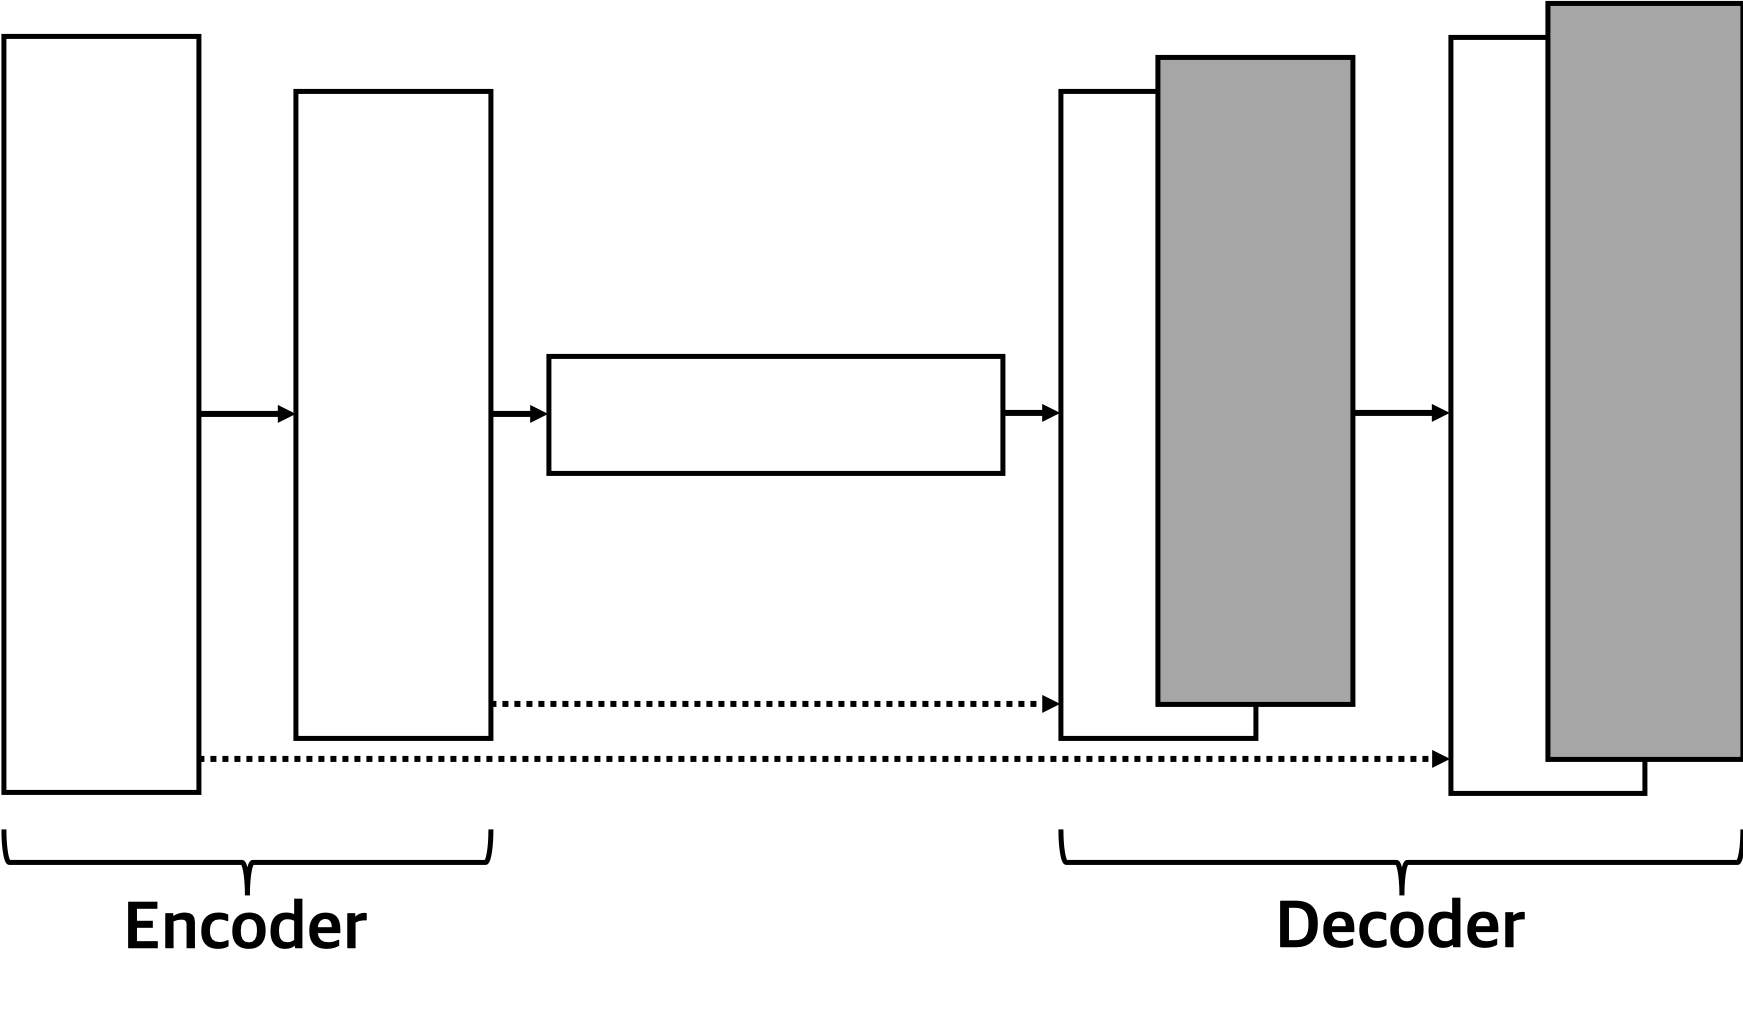
\includegraphics[width=0.6\textwidth]{unet}
	\caption{Encoder - Decoder Network에서 skip-connection의 역할. 점선 화살표로 표시된 부분이 skip-connection이다.}
	\label{fig:unet}
\end{figure}


\subsection{Discriminator}

Discriminator에 대해선, \pixpix~논문에서 사용된 PatchGAN을 사용하였다.
일반적인 discriminator가 주어진 이미지를 크기가 1 x 1이 될 때까지 줄인다음에 진짜 이미지인지 가짜 이미지인지 판별하는 반면, PatchGAN은 원래 이미지의 특정 \textit{patch}를 커버하게 하는 discriminator이다.
예를 들어, 256 x 256 크기의 이미지가 들어오면, convolutional layer를 통해 이미지의 크기가 30 x 30이 될 때까지 줄이면, 이 줄어든 이미지의 한 픽셀은 원래 이미지의 대략 70 x 70 크기의 patch에 대한 정보를 커버한다고 볼 수 있다.
또한,이미지의 크기가 1 x 1이 될 때까지 줄이는 discriminator는 한 픽셀이 전체 이미지의 정보를 다 갖는 PatchGAN으로 볼 수 있다.
비록 \stylepaint 에서는 저자들이 PatchGAN을 사용하면 완벽한 채색은 힘들다고 주장했지만, 구현 정보의 부재로 인하여 일단은 우리는 \pixpix 에서 가장 좋은 결과를 낸다고 주장하는 70 x 70 PatchGAN을 사용하여 실험을 진행하였다.